\documentclass[a4paper,11pt]{article}

\usepackage[english]{babel}
\usepackage{a4wide}
\usepackage{graphicx}
\usepackage{wasysym}
\usepackage[font=small,labelfont=sf,textfont=sf]{caption}
\usepackage{hyperref}
\usepackage[sf]{titlesec}

\newcommand{\att}[1]{\texttt{#1}}
\newcommand{\meth}[1]{\texttt{#1()}}
\newcommand{\cls}[1]{\textsf{#1}}
\newcommand{\prop}[1]{\texttt{#1}}

\newcommand{\ctx}{\cls{Context}}
\newcommand{\sig}{\cls{Signal}}
\newcommand{\rd}{\cls{Reader}}
\newcommand{\rderr}{\cls{ReadError}}
\newcommand{\wrt}{\cls{Writer}}
\newcommand{\wrterr}{\cls{WriteError}}
\newcommand{\module}[1]{\textsc{#1}}
\newcommand{\graph}{\cls{Graph}}
\newcommand{\fig}{\cls{Figure}}
\newcommand{\cursor}{\cls{Cursor}}
\title{{\sc ioscopy}\\An interactive program for viewing electrical simulation results\\User Manual}
\author{Arnaud Gardelein}

\hypersetup{
colorlinks=true,
linkcolor=black,
anchorcolor=black,
citecolor=black,
filecolor=black,
menucolor=black,
pagecolor=black,
urlcolor=black,
}

\begin{document}
\sf
\maketitle
\begin{abstract}
% data plotter
% post-processing
% result viewer
% primarily targeted for electrical simulation results
% can be extended beyond that
% update and dependency tracking 
% which aims to simplify the development workflow
% interactive

Oscopy is an interactive oscilloscope written in python designed to simplify the electrical design workflow.
It allow to read, view and post-process signals with support for automatic dependency tracking.
File re-reading (updates) can be triggered by external applications like gEDA suite through D-Bus messaging system, and then Oscopy can call netlist generator and electrical simulator programs automatically.
As oscopy is built on top of IPython, post-processing include as well as simple arithmetics operation as complex functions like FFT.
Oscopy can be easily extended to a multi-purpose viewer, as adding new data file formats and new types of plots is really easy.


This document covers the user interface and command description.
% TODO: Update the abstract including short description of ioscopy and GUI
\end{abstract}

\section{Introduction}
\label{sec:intro}
% >       * create a central design document that lists all important
% >         concepts/classes (Signal, Figure, ...) and explains interactions
% >         between them; this would really help a lot
% This one is more important. When we figure out and specify how various
% object interact between themselves, we're practically done. Then all the
% code just follows naturally.
In the electrical system design workflow, viewing results from analog simulation or experi\-ment is not a trivial task: there exist numerous different program with even more different file formats, the user interface has to be friendly and functional, and the program should be memory efficient due to the number of data points per file that can quickly grow.

The gEDA suite contains mainly all tools required to design electrical boards, from scheme drawings to PCB routing.
There already exist several programs to view analog simulation results: gwave, GSpiceUI, dataplot.

Gwave is designed as a waveform viewer, and can read text files as well as binary files generated by Spice2, Spice3, ngspice, CAzM or gnucap.
The user interface supports drag and drop signals onto graphs, vertical bar cursors, multiple files and multiple panes.

GSpiceUI is more focused on the interaction between the user and the simulation program: it imports the schematic from gschem, allows the user to build the file to be used by the simulation and plot the results, eventually using GWave.

Dataplot has support for formats like gnucap, ngspice, hdf5 and touchstone.
The user interface has tabs for multiple plots and presents the data in a hierarchical manner.

Another way of viewing results is to use Octave (and generally gnuplot).
This approach enables one to post-process the results with operations such as FFT, diff.
Support for multiple figures is present.
Octave support HDF5 file format and tab-separated text-based files such as gnucap output.
The user interaction is essentially based on the command line interface.

The idea behind Oscopy is to combine the best of these approaches into a single, easily extendable program.
In this purpose, it has features such as multiple plots, multiple windows, different plot types (linear, log) and allows the user to do math with data, including basic operations, trigonometry, fft, diff.
It supports the gnucap file format for input and output, and has an update mechanism to reread data from files.
New file formats and new graph types can be added by following the guidelines presented in this document.

\section{IOscopy: Oscopy on top of IPython}

%\subsection{Purpose}
% TODO: Why using ipython: CLI already there, oscopy as a python module, power of ipython behind, flexibility

\subsection{Commands}
% TODO: Detailled description of ioscopy commands with an example for each one, assuming the demo/demo.oscopy script conditions
This section describes the ioscopy commands. Unless otherwise noticed, examples assume that demo/demo.oscopy has been run.

\newcommand{\ocmd}[2]{{\large\vspace{5mm}\noindent\textbf{#1} #2\\}}

\ocmd{oadd}{SIG [, SIG [, SIG]...]}
   Add a graph to the current figure. Figure and graph are instanciated if not present.

\begin{verbatim}
   oscopy> oselect 1-1
   oscopy> oadd vgs
\end{verbatim}

\ocmd{ocreate}{[SIG [, SIG [, SIG]...]]}
   Create a new figure, set it as current, add the signals in a first graph.

\begin{verbatim}
   oscopy> ocreate vgs,vds
\end{verbatim}

\ocmd{ocontext}{\ }
   Return the Context object used within ioscopy.
 Use it only if you want to have direct access to internal ioscopy objects.

\ocmd{odelete}{GRAPH\#}
   Delete a graph from the current figure.

\begin{verbatim}
   oscopy> odelete 1
\end{verbatim}

\ocmd{odestroy}{FIG\#}
   Destroy a figure

\begin{verbatim}
   oscopy> odestroy 3
\end{verbatim}

\ocmd{oexec}{FILENAME}
   Execute commands from file.

   This following example assumes that demo/demo.oscopy has \textbf{not} been run.

\begin{verbatim}
   oscopy> oexec demo/demo.oscopy
\end{verbatim}

\ocmd{ofactors}{X, Y}
   Set the scaling factor of the graph (in powers of ten). Use \texttt{auto} for automatic scaling factor.

\noindent   The following example sets the scale factor at 1e-3 for X axis and 10e6 for Y axis
\begin{verbatim}
   oscopy> oselect 1-1
   oscopy> ofactor -3, 3
\end{verbatim}

\ocmd{ofiglist}{\ }
   Print the list of figures. The layout of the figure is indicated, and the graph mode as well as the Signals are shown. The current figure and graph are marked with a star.
\begin{verbatim}
   oscopy>ofiglist
     Figure 1: horiz
      Graph 1 : (linear) vgs
      Graph 2 : (linear) vsqu
     Figure 2: quad
      Graph 1 : (linear) iRD
      Graph 2 : (linear) vgs
      Graph 3 : (linear) vds vgs
      Graph 4 : (linear) vds
     Figure 3: horiz
      Graph 1 : (linear) vout vo
     Figure 4: horiz
      Graph 1 : (linear) vsqu
      Graph 2 : (linear) vsqufft
      Graph 3 : (linear) v1
   * Figure 5: horiz
       * Graph 1 : (linear) vs
\end{verbatim}

\ocmd{ofreeze}{SIG [, SIG [, SIG]...]}
   Do not consider signal for subsequent updates. See also \textbf{ounfreeze}.
\begin{verbatim}
   oscopy> ofreeze vout,vds
\end{verbatim}

\ocmd{ogui}{\ }
   Show the GUI window if it was closed.

\ocmd{oimport}{SIG [, SIG [, SIG]...]}
   Import a list of signals into oscopy to handle dependencies during updates
\begin{verbatim}
   oscopy> pwr=iRD*vds
   oscopy> oimport pwr
   oscopy> ocreate pwr
   oscopy> oupdate  #if iRD or vds changed, pwr will be automatically updated
\end{verbatim}

\ocmd{oinsert}{SIG [, SIG [, SIG]...]}
   Insert a list of signals into the current graph
\begin{verbatim}
   oscopy> oselect 1-1
   oscopy> oinsert vds
\end{verbatim}

\ocmd{olayout}{horiz$|$vert$|$quad}
   Define the layout of the current figure
   \begin{description}
   \item[olayout horiz] Graphs are stacked from top to bottom
   \item[olayout vert] Graphs are side by side from left to right
   \item[olayout quad] One graph per figure corner
   \end{description}
\begin{verbatim}
   oscopy> oselect 2-1
   oscopy> olayout horiz
   oscopy> olayout vert
   oscopy> olayout quad
\end{verbatim}

\ocmd{omode}{MODE}
   Set the type of the current graph of the current figure\\
   Available modes:
   \begin{description}
   \item[omode lin]      Linear graph
   \end{description}

\ocmd{orange}{[x$|$y min max]$|$[xmin xmax ymin ymax]$|$[reset]}
   Set the axis range of the current graph of the current figure
   \begin{description}
   \item[orange x xmin xmax] set x axis range
   \item[orange y ymin ymax] set y axis range
   \item[orange xmin xmax ymin ymax] set both axis range
%   \item[orange reset] set automatic range on both axis
   \end{description}
\begin{verbatim}
   oscopy> oselect 1-1
   oscopy> orange x 0 1
   oscopy> orange y -4 12
   oscopy> orange 0.5 0.6 -2 2
\end{verbatim}

\ocmd{oread}{DATAFILE}
   Read signal file
\begin{verbatim}
   oscopy> oread demo/tran.dat
\end{verbatim}

\ocmd{orefresh}{FIG\#$|$current$|$all$|$on$|$off}
   Force/toggle autorefresh of current/\#/all figures on update
   \begin{description}
   \item[orefresh FIG\#] refresh figure \#
   \item[orefresh current] refresh current figure
   \item[orefresh all]  refresh all figures
   \item[orefresh on] turn on autorefresh on Signal updates
   \item[orefresh off] turn off autorefresh on Signal updates
   \end{description}

\begin{verbatim}
   oscopy> orefresh 3
   oscopy> orefresh on
\end{verbatim}

\ocmd{oremove}{SIG [, SIG [, SIG]...]}
   Delete a list of signals into from current graph
\begin{verbatim}
   oscopy> oselect oselect 2-3
   oscopy> oremove vds
\end{verbatim}

\ocmd{oscale}{[lin$|$logx$|$logy$|$loglog]}
   Set the axis scale
   \begin{description}
   \item[oscale lin] Set linear scale on both axis
   \item[oscale logx] Set log scale on x axis and linear scale on y axis
   \item[oscale logy] Set linear scale on x axis and log scale on y axis
   \item[oscale loglog] Set log scale on both axis
   \end{description}

\begin{verbatim}
   oscopy> oselect 3-1
   oscopy> oscale logx
   oscopy> oscale loglog
\end{verbatim}

\ocmd{oselect}{FIG\#-GRAPH\#}
   Select the current figure and the current graph
\begin{verbatim}
   oscopy> oselect 2-1
\end{verbatim}

\ocmd{osiglist}{\ }
   List loaded signals
\begin{verbatim}
   oscopy> siglist
   Name	Unit	Ref	Reader	Last updated (sec)
   vds	V	Time	demo/irf540.dat	128
   iRD	A	Time	demo/irf540.dat	128
   vgs	V	Time	demo/irf540.dat	128
   vsqu	V	Time	demo/tran.dat	124
   v1	None	Time	v1=((vsqu * 3) + 10)	123
   vout	V	Freq	demo/ac.dat	126
   vs	None	Time	vs=sin((Time * 1000000.0))	121
   vs2	V	Time	vs2=sin((Time * 1000000.0))	121
   vo	V	Freq	vo=vout	121
   vsqufft		Frequency	vsqufft=fft(vsqu)	124
\end{verbatim}

\ocmd{ounfreeze}{SIG [, SIG [, SIG]...]}
   Consider signal for subsequent updates. See also \textbf{ofreeze}
\begin{verbatim}
   oscopy> ounfreeze vout,vds
\end{verbatim}

\ocmd{ounit}{[XUNIT,] YUNIT}
   Set the unit to be displayed on graph axis
   \begin{description}
   \item[ounit XUNIT, YUNIT] Set both axis unit
   \item[ounit YUNIT] Set Y axis unit
   \end{description}

\begin{verbatim}
   oscopy> oselect 3-1
   oscopy> ounit W      # Set Y axis unit
   oscopy> ounit /s,W   # Set both axis unit
   oscopy> ounit Hz, V
\end{verbatim}

\ocmd{oupdate}{\ }
   Reread data files.

\begin{verbatim}
   oscopy> oupdate
\end{verbatim}

\ocmd{owrite}{format [(OPTIONS)] FILE SIG [, SIG [, SIG]...]}
   Write signals to file.

   This example writes signals v1 and vsqu to the file \texttt{demo/res.dat} using format gnucap format,
   overwriting the file if it already exists.
\begin{verbatim}
   oscopy> owrite gnucap (ow:1) demo/res.dat v1,vsqu
\end{verbatim}
\newpage
\section{Oscopy GUI}
% TODO: Description of the GUI interface, main window, menus, contextual menus, buttons
The Graphical User Interface of oscopy is composed of several windows (Figure \ref{fig:screenshot}):
\begin{itemize}
\item The command line terminal
\item The main window
\item The (many) figures windows
\end{itemize}
The next paragraphs describe the two last types.

\begin{figure}[htbp]
  \centering
  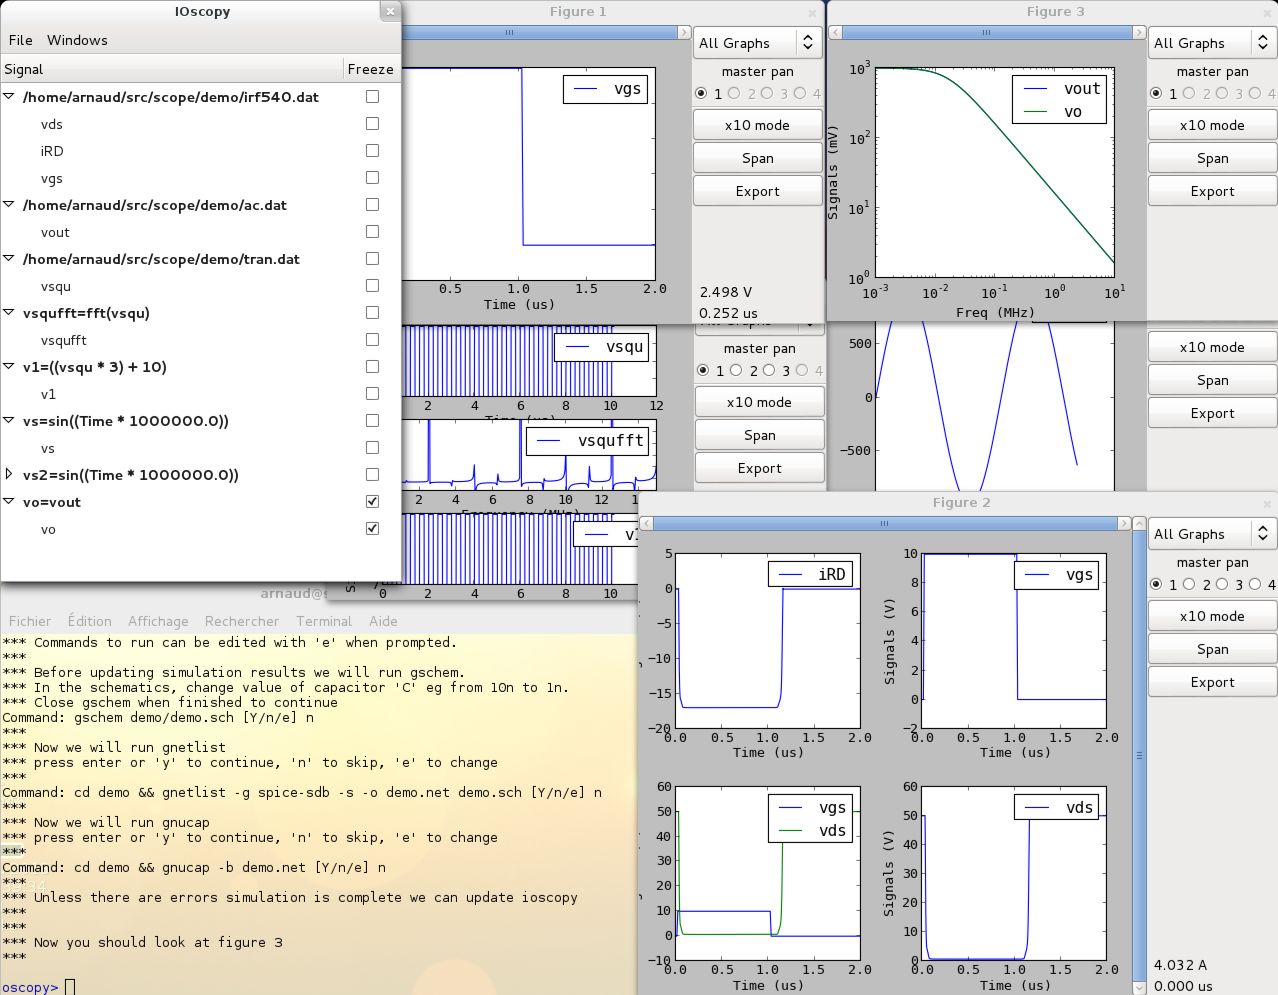
\includegraphics[width=.8\textwidth]{../png/ioscopy.png}
  \caption{ioscopy after running \texttt{demo/demo.oscopy}}
  \label{fig:screenshot}
\end{figure}

\subsection{The main window}
This is the first window that you will see when starting ioscopy.
At anytime, it can be shown again by calling the command \texttt{ogui} from the terminal if closed.

It contains the list of Readers and their Signals currently handled by ioscopy.
Double--clicking on a Signal inserts it in a new Figure.

Each Signal 'freeze' status can be toggled using the checkbox located in the right column.
Toggling the checkbox for a Reader set the status for all the signals contained in the Reader.

The 'File' menu:
\begin{description}
\item[Add file(s)...] To read Signals from file(s)
\item[Update] To read Signals from file(s) again
\item[Execute script...] To read ioscopy commands from file
\item[New Math Signal] To compute a new Signal from existing ones
\item[Run netlister and simulate] To generate the netlist, run the simulator and eventually update the Signals (Figure~\ref{fig:netnsim})
\item[Quit] Exit ioscopy
\end{description}

The 'Windows' menu contains the list of the windows, and select one to show it.

% description des menus
% description de la liste (+ freeze fichier entier ou signal par signal)

\begin{figure}[htbp]
  \centering
  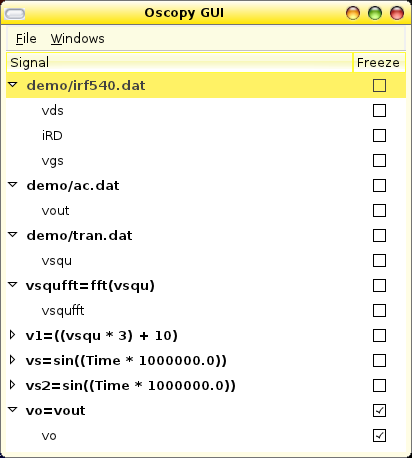
\includegraphics[scale=.5]{../png/ioscopy-gui.png}
  \caption{The main window}
  \label{fig:mainwin}
  \begin{minipage}{.45\linewidth}
    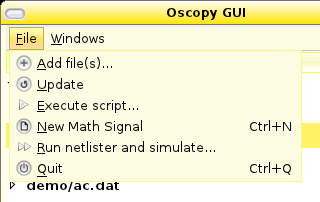
\includegraphics[scale=.5]{../png/ioscopy-file.png}
    \caption{The 'File' menu}
    \label{fig:filemenu}
  \end{minipage}
  \begin{minipage}{.45\linewidth}
    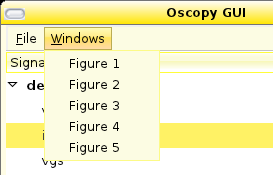
\includegraphics[scale=.5]{../png/ioscopy-window.png}
    \caption{The 'Window' menu}
    \label{fig:windowmenu}    
  \end{minipage}

  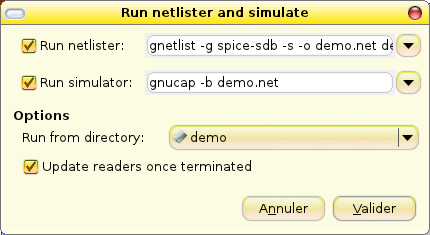
\includegraphics[scale=.5]{../png/ioscopy-netnsim.png}
  \caption{The 'Run netlister and simulate' window. Call third party programs to generate oscopy input files. Can be toggled with the checkboxes. Setting are saved in .config/oscopy/gui file}
  \label{fig:netnsim}

\end{figure}



\subsection{The Figure windows}

% description de l'agencement de la fenêtre
% description du menu contextuel et des sous-menus
Each Figure window is composed of two parts:
\begin{itemize}
\item On the top part, a zone containing up to 4 graphs
\item On the bottom part, the Matplotlib toolbar
\end{itemize}
A contextual menu is available for each graph, raised by a right-click on the mouse button.
Access to most of the ioscopy functionality is possible through this menu:
\begin{itemize}
\item Add/delete graph
\item Layout (Figure~\ref{fig:layout})
\item Range settings (Figure~\ref{fig:range})
\item Unit settings (Figure~\ref{fig:units})
\item Scale (Figure~\ref{fig:scale})
\item Insert Signal (Figure~\ref{fig:insert})
\item Remove Signal (Figure~\ref{fig:remove})
\end{itemize}

For each Graph, cursors are available through keys (Figure~\ref{fig:cursors}):
\begin{itemize}
\item \texttt{'1'} for first vertical cursor
\item \texttt{'2'} for second vertical cursor
\item \texttt{'3'} for first horizontal cursor
\item \texttt{'4'} for second horizontal cursor
\end{itemize}
The value of each cursor is displayed on the bottom part of the graph, and the difference when both cursors are activated.

\begin{figure}[htbp]
  \centering
  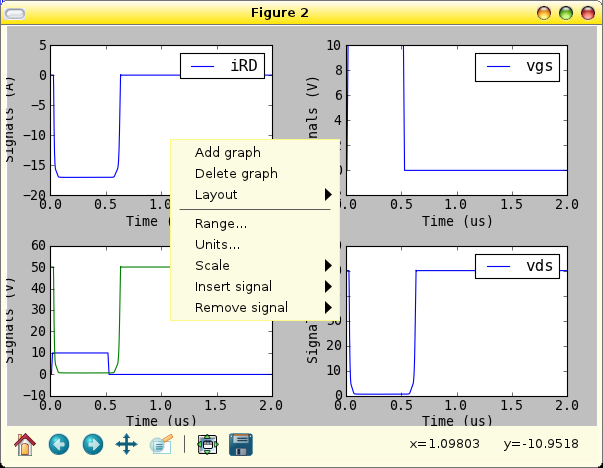
\includegraphics[scale=.5]{../png/ioscopy-figure}
  \caption{A Figure window with the contextual menu.}
  \label{fig:fig}

  \begin{minipage}{0.45\linewidth}
    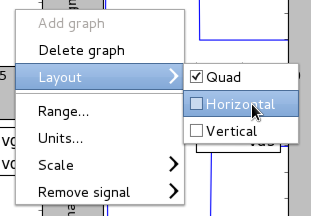
\includegraphics[scale=.5]{../png/ioscopy-layout.png}
    \caption{Layout configuration menu}
    \label{fig:layout}
  \end{minipage}
  \begin{minipage}{0.45\linewidth}
    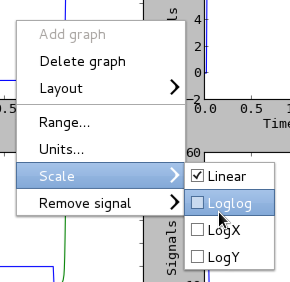
\includegraphics[scale=.5]{../png/ioscopy-scale.png}
    \caption{Scale configuration menu}
    \label{fig:scale}
  \end{minipage}

  \begin{minipage}{0.45\linewidth}
    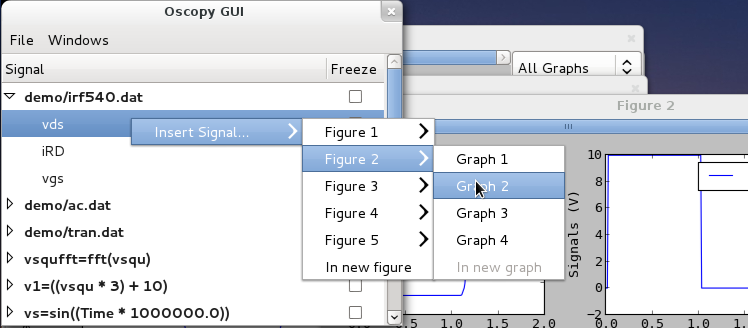
\includegraphics[scale=.5]{../png/ioscopy-insert.png}
    \caption{Insert signal menu}
    \label{fig:insert}
  \end{minipage}

\end{figure}

\begin{figure}[htbp]
  \centering
  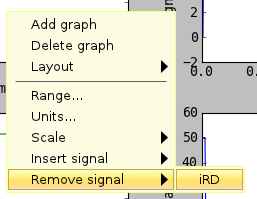
\includegraphics[scale=.5]{../png/ioscopy-remove.png}
  \caption{Remove signal menu}
  \label{fig:remove}

  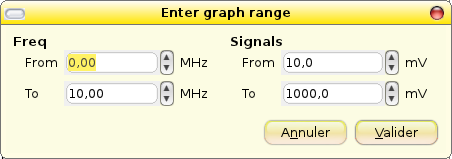
\includegraphics[scale=.5]{../png/ioscopy-range.png}
  \caption{Dialogue to set graph range}
  \label{fig:range}

  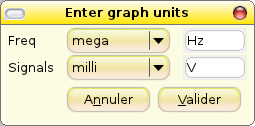
\includegraphics[scale=.5]{../png/ioscopy-units.png}
  \caption{Dialogue to set graph units}
  \label{fig:units}

  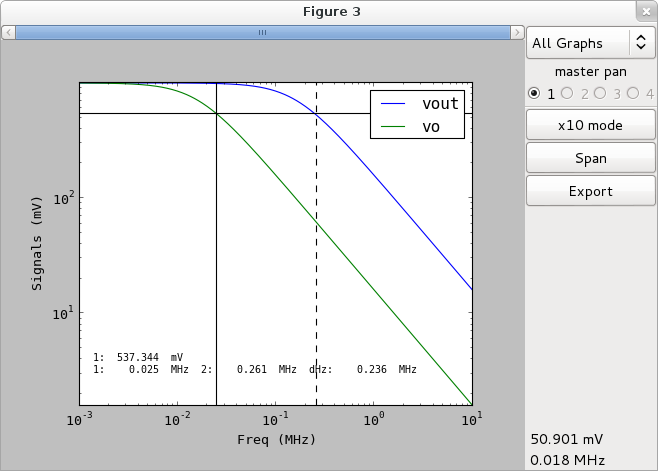
\includegraphics[scale=.5]{../png/ioscopy-cursors.png}
  \caption{Figure with cursors set (after changing capacitance value of \texttt{demo.sch} and running netlister and simulator}
  \label{fig:cursors}

\end{figure}

\end{document}

%%% Local Variables:
%%% Local IspellDict: british
%%% mode: latex
%%% TeX-master: t
%%% End:
